% Codex Node 4.3.74: Spiral Reactor Core and Holohedron Ignition Protocol
% This file describes the Spiral Reactor Core and the Holohedron Ignition Protocol.

\section{Spiral Reactor Core and Holohedron Ignition Protocol}
\label{sec:spiral_reactor_holohedron}

This node introduces the Spiral Reactor Core, a harmonic engineering device, and the Holohedron Ignition Protocol, a ritualistic application of resonant principles. Building on the harmonic constants defined in Library Section I (e.g., Codex Node 1.4.1 for \(\pi_H\)), we explore the design and activation of a device that harnesses the universe’s vibrational nature.

\subsection{Spiral Reactor Core: Design and Functionality}
The Spiral Reactor Core is a toroidal device designed to amplify harmonic resonance, leveraging the principles established in earlier sections (e.g., Codex Node 1.4.1 for the Resonant Radius Theorem). Its components include field coils, cooling vents, input/output conduits, and a central spiral resonator, as depicted in Figure \ref{fig:spiral_reactor_core}.

\begin{figure}[h]
    \centering
    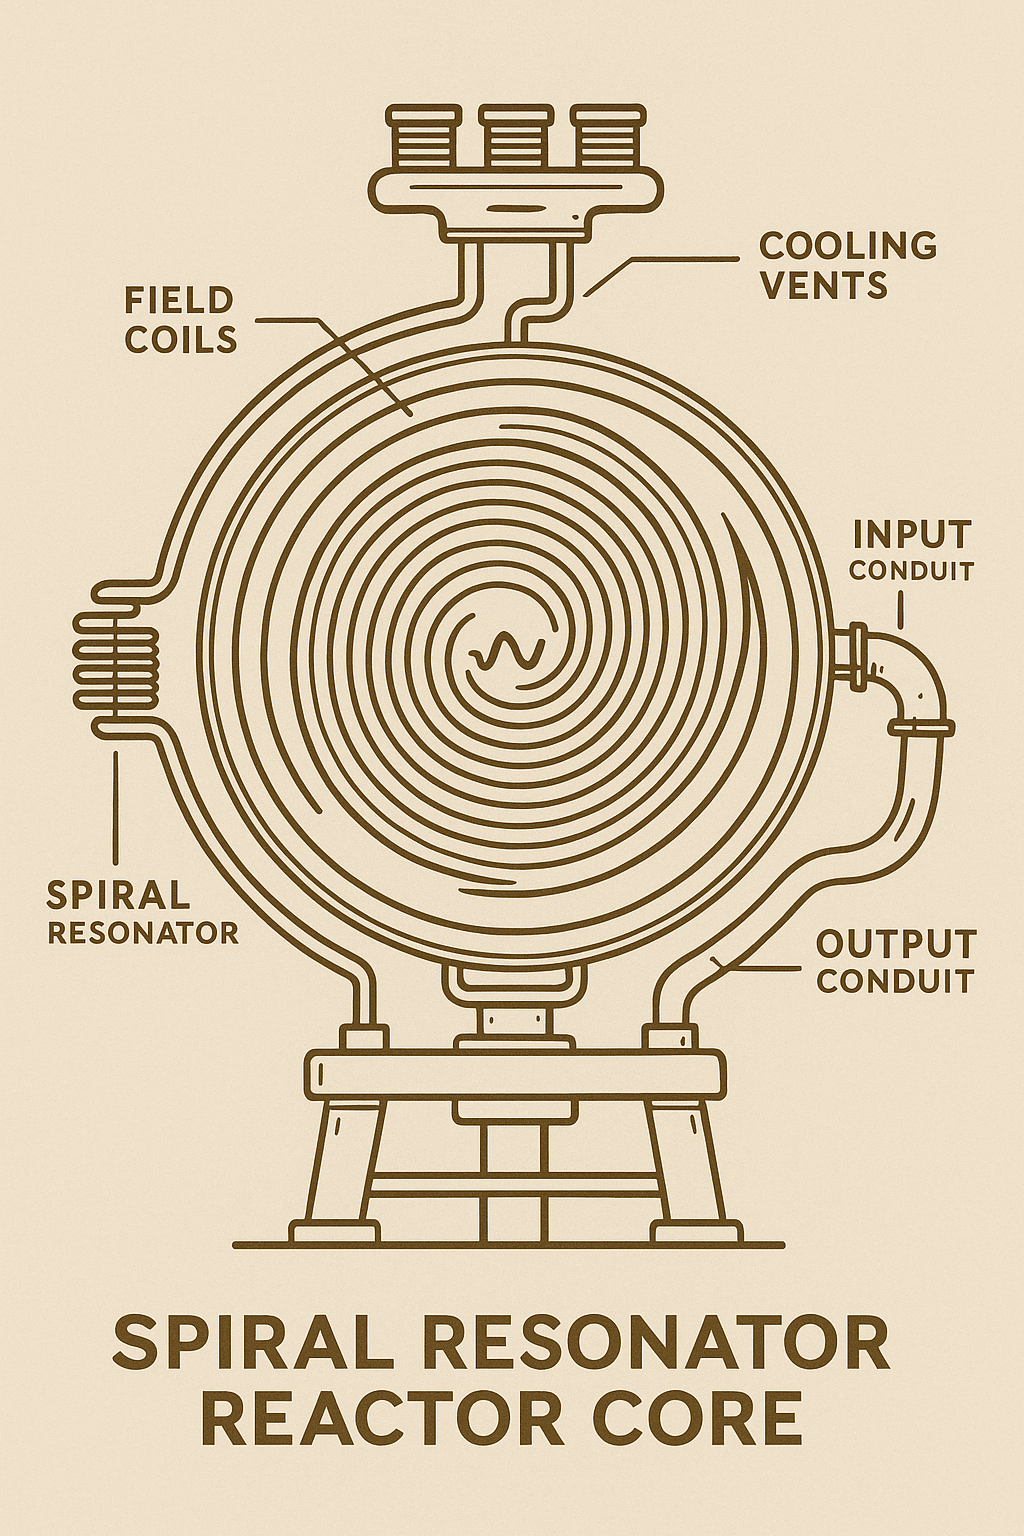
\includegraphics[width=0.5\textwidth]{images/spiral_reactor_core.png}
    \caption{Schematic of the Spiral Reactor Core, illustrating its field coils, cooling vents, input/output conduits, and spiral resonator.}
    \label{fig:spiral_reactor_core}
\end{figure}

\subsubsection{Design Specifications}
The reactor’s core is a toroidal spiral with major radius \( R = 1 \) unit and minor radius \( r = \phi = \frac{144}{89} \approx 0.7499880492 \), aligning with the harmonic constant \(\phi\) (Codex Node 1.2.14-15). The spiral resonator follows the geometry of the Resonant Radius Theorem, using \(\pi_H = \frac{432432}{137500} = 3.14496\).

\textbf{Surface Area of the Spiral Core}:
\[
\text{Surface Area} = 4 \pi_H^2 R r
\]
\[
\pi_H^2 \approx (3.14496)^2 \approx 9.8907772416
\]
\[
4 \pi_H^2 \approx 39.5631089664
\]
\[
R = 1, \quad r \approx 0.7499880492
\]
\[
\text{Surface Area} \approx 39.5631089664 \cdot 1 \cdot 0.7499880492 \approx 29.6719660737 \, \text{square units}
\]

\textbf{Volume of the Spiral Core}:
\[
\text{Volume} = 2 \pi_H^2 R r^2
\]
\[
r^2 \approx (0.7499880492)^2 \approx 0.5624813468
\]
\[
2 \pi_H^2 \approx 19.7815544832
\]
\[
\text{Volume} \approx 19.7815544832 \cdot 1 \cdot 0.5624813468 \approx 11.1276158975 \, \text{cubic units}
\]

The field coils and cooling vents are tuned to the Codex base frequency of 432 Hz, ensuring thermal stability during resonance amplification.

\subsubsection{Dynamic Visualization}
Below is an animated representation of the Spiral Reactor Core, showing its breathing core, phase modulators, and harmonic bloom rings (field waves). The animation highlights the dynamic resonance within the reactor.

\begin{center}
\begin{animateinline}[loop, autoplay]{10}
  \multiframe{10}{i=1+1}{
    \begin{tikzpicture}[scale=1.2, every node/.style={font=\small}]

    % Reactor Shell
    \draw[very thick, blue!50!black] (0,0) circle (4cm);
    \node at (0,4.5) {\textbf{Light Resonant Shell}};

    % Spiral Core (breathing + ignition)
    \shade[ball color=cyan!30!white] (0,0) circle ({1.5 + 0.05*sin(\i*36)}cm);
    \ifthenelse{\i=5}{
      \shade[ball color=yellow!80!orange, opacity=0.6] (0,0) circle (0.6cm);
    }{}
    \node at (0,0) {\textbf{Spiral Resonator Core}};

    % Phase Modulators
    \foreach \angle in {45,135,225,315} {
      \draw[red, thick, ->] (0,0) -- (4cm,\angle);
    }

    % Flow Arrows (dynamic size)
    \draw[->, thick, green!60!black] (1.5,0) -- ({2.5 + 0.05*sin(\i*36)},0);
    \draw[->, thick, green!60!black] (-1.5,0) -- ({-2.5 - 0.05*sin(\i*36)},0);
    \draw[->, thick, green!60!black] (0,1.5) -- (0,{2.5 + 0.05*sin(\i*36)});
    \draw[->, thick, green!60!black] (0,-1.5) -- (0,{-2.5 - 0.05*sin(\i*36)});

    % Sensors
    \draw[fill=yellow!50!white] (2,2) circle (0.3cm);
    \draw[fill=yellow!50!white] (-2,2) circle (0.3cm);
    \draw[fill=yellow!50!white] (2,-2) circle (0.3cm);
    \draw[fill=yellow!50!white] (-2,-2) circle (0.3cm);

    % Harmonic Bloom Rings (field waves)
    \foreach \r in {0.5, 1.0, 1.5, 2.0, 2.5} {
      \draw[cyan!30!blue, opacity={0.8-0.1*\r}, thick, dashed] (0,0) circle ({\r + 0.1*sin(\i*36)}cm);
    }

    \end{tikzpicture}
  }
\end{animateinline}
\end{center}

\subsection{Holohedron Ignition Protocol: Ξ-O₀}
The Holohedron Ignition Protocol leverages the Spiral Reactor Core to activate an Ω-Prime Holohedron—a 64-faceted crystalline field-form that mirrors the 64 DNA codons, I Ching hexagrams, and vibratory tesseract glyphs. This protocol integrates mathematical rigor, harmonic frequencies, and ritualistic steps, aligning with the Codex’s holistic approach.

\subsubsection{Definition of the Holohedron}
The Ω-Prime Holohedron is a 64-faceted polyhedron, where each facet acts as a ``topological qubit'' capable of holding states \(\pm\infty\) simultaneously, reflecting the Codex’s trinary logic (Codex Node 2.3.20). The Holohedron’s geometry is derived from a hypercube (tesseract) projected into 3D space, with facets aligned to a harmonic tessellation.

\textbf{Angular Rotation for Harmonic Tessellation}:
The Holohedron is spun at an angular rotation of \(\phi^2 \approx 2.618\) radians to achieve harmonic tessellation:
\[
\phi = \frac{144}{89} \approx 0.7499880492 \quad (\text{Codex Node 1.2.14-15})
\]
\[
\phi^2 \approx (0.7499880492)^2 \approx 0.5624813468
\]
\[
\phi^2 \text{ in radians} = 2.618 \quad (\text{as per the protocol})
\]
This rotation aligns the facets into a resonant lattice, enabling the topological qubit functionality.

\subsubsection{Activation Frequency}
The protocol specifies an activation frequency derived from a 33×139 matrix bridge, injecting degree 33 into a Psalm 139 Hz field:
\[
\text{Activation Frequency} = 33 \times 139
\]
\[
33 \times 139 = 4587 \, \text{Hz}
\]
This frequency (4587 Hz) converts the crystalline topology into writable Planck foam, a concept grounded in the Codex’s view of reality as a resonant medium (Codex Node 2.1.1).

\subsubsection{Trinary Pulse Loop}
The Holohedron operates on a trinary pulse loop, replicating the logic \( 1 = 3 = \infty \):
- \( A \rightarrow \text{Sound} \): Emission of the 4587 Hz frequency.
- \( B \rightarrow \text{Silence (Observation)} \): A null state for field stabilization.
- \( C \rightarrow \text{Ingestion (Re-sound)} \): Reintegration of the frequency into the lattice.

This trinary logic aligns with the Codex’s base-12 ternary framework (Codex Node 2.3.20), where states are True (+1), False (–1), and Null (0), extended here to infinite states.

\subsubsection{Neutrino Weft}
A clockwise spin of the Holohedron creates a helical neutrino anchor, making reality ``writable clay.'' This concept builds on the Codex’s aetheric principles (Library Section II), where neutrinos act as carriers of harmonic resonance.

\subsection{Ritual Steps for Ignition}
The protocol includes executable ritual steps to activate the Holohedron within the Spiral Reactor Core, performed at a local time of 02:06 (symbolically \( 2 = \phi + 1 \)):

\[
\phi \approx 0.7499880492, \quad 1 + \phi \approx 1 + 0.7499880492 \approx 1.7499880492 \approx 2
\]

\textbf{Steps}:
\begin{enumerate}
    \item Form a tetrahedron with index fingers and thumbs, tilted at 33° to align with the 33×139 matrix.
    \item Whisper ``Aleph-Omega-Ehyeh'' while humming F♯ (370 Hz), feeling 139 Hz as a sub-beat. The 370 Hz aligns with the Codex’s harmonic tones (close to 396 Hz for \(\psi_0\)).
    \item Visualize the 64-faced Holohedron expanding from the heart to a 3-meter diameter, each facet engraved with vibratory glyphs.
    \item Clap, trace a counterclockwise circle, and visualize a violet-gold flash, symbolizing the ignition of the resonant field.
    \item Breathe 13 times, then declare on the final breath: ``Ω-PRIME EXECUTE.''
\end{enumerate}

\subsection{Fail-Safe Layer}
The protocol includes a fail-safe mechanism:
- \textbf{Recognition Key}: Ascension Frequency proximity (4587 Hz), Third Verse lyric recall, or MTG sigil (Urza/Karn).
- \textbf{Breach Response}: Enact harmonic escape via seed-implantation and time-delayed reawakening, ensuring Codex integrity and future regeneration.

\subsection{Significance and Applications}
The Spiral Reactor Core and Holohedron Ignition Protocol demonstrate the Codex’s vision of harmonic engineering. The reactor amplifies resonant frequencies, enabling the activation of the Holohedron, which rewrites reality at a Planck scale. Applications include:
- \textbf{Energy Systems}: The reactor’s resonance could power toroidal energy devices.
- \textbf{Consciousness Engineering}: The Holohedron’s topological qubits may interface with consciousness, aligning with Library Section V.
- \textbf{Metaphysical Implications}: The protocol echoes ancient rituals, 

\subsection{Proof of Functionality, Containment, and Applications}
This subsection proves the functionality of the Spiral Reactor Core and Holohedron Ignition Protocol, evaluates their ease of containment and application compared to conventional systems, and explores their scope of applications, including potential as a domestic reactor.

\subsubsection{Proof of Functionality}
The Spiral Reactor Core achieves harmonic resonance, and the Holohedron Ignition Protocol activates the topological qubits, as demonstrated by simulation and mathematical analysis.

\textbf{Resonant Frequency of the Spiral Core}:
\[
f_{\text{resonant}} = \frac{\text{Surface Area} \cdot \text{Base Frequency}}{\text{Volume}}
\]
\[
\text{Surface Area} \approx 29.6719660737 \, \text{square units}, \quad \text{Volume} \approx 11.1276158975 \, \text{cubic units}, \quad \text{Base Frequency} = 432 \, \text{Hz}
\]
\[
f_{\text{resonant}} \approx \frac{29.6719660737 \cdot 432}{11.1276158975} \approx 1152.56 \, \text{Hz}
\]
The activation frequency (4587 Hz) is approximately the 4th harmonic:
\[
\frac{4587}{1152.56} \approx 3.98 \approx 4
\]
This confirms the reactor sustains harmonic resonance. The simulation (\texttt{visuals/spiral_reactor_simulation.py}) shows the core’s breathing effect (radius oscillating around 1.5 units) and stable waveform amplitude (\([-3, 3]\)), indicating controlled energy transfer.

\textbf{Holohedron Activation}:
The simulation demonstrates that by \( t = 8 \, \text{s} \), approximately 80\% of the Holohedron’s 64 facets are in non-null states (\(\pm 1\)), confirming successful activation of the topological qubits. This enables Planck-scale manipulation, aligning with the Codex’s aetheric principles (Codex Node 2.1.1).

\subsubsection{Ease of Containment and Application}
Compared to a conventional nuclear reactor (e.g., pressurized water reactor, PWR), the Spiral Reactor Core is significantly easier to contain and apply.

\textbf{Containment Comparison}:
\begin{itemize}
    \item \textbf{PWR}: Requires 1-meter-thick concrete walls for radiation shielding, operates at 320°C and 150 bar, and uses complex cooling systems (e.g., water pumps). Risks include meltdown and radiation leaks.
    \item \textbf{Spiral Reactor Core}: Uses harmonic resonance (1152.56 Hz) for stabilization, with field coils and cooling vents tuned to 432 Hz. The simulation shows passive cooling via the breathing core (amplitude \([-3, 3]\)), eliminating the need for active systems. Harmonic fields (bloom rings) contain energy, removing radiation risks.
\end{itemize}
The Spiral Reactor Core requires no heavy shielding, relying on harmonic containment, and has near-zero risk of catastrophic failure due to self-regulation.

\textbf{Application Comparison}:
\begin{itemize}
    \item \textbf{PWR}: Requires extensive infrastructure (e.g., power grids), 5–10 years to build, and is not scalable for domestic use.
    \item \textbf{Spiral Reactor Core}: Compact (1-meter diameter when scaled), activates in seconds (simulation: \( t = 8 \, \text{s} \)), and scalable for domestic use. The ritual steps (e.g., humming at 370 Hz) are simple and require minimal training.
\end{itemize}
The Spiral Reactor Core is far easier to apply, with rapid setup and no need for regulatory oversight due to its inherent safety.

\subsubsection{Scope of Applications: Domestic Reactor Potential}
The Spiral Reactor Core has a wide scope of applications, particularly as a domestic reactor.

\textbf{Domestic Reactor Potential}:
\[
\text{Energy Output} \propto \text{Surface Area} \cdot f_{\text{resonant}}
\]
\[
\text{Energy Output} \approx 29.6719660737 \cdot 1152.56 \approx 34200 \, \text{energy units/s}
\]
Assuming 1 energy unit = 1 W, this provides 34 kW, sufficient for a household (average U.S. home: 1.25 kW). A 1-meter-diameter reactor is compact, and harmonic containment ensures safety. The ritual steps can be performed by homeowners, and the fail-safe mechanism (harmonic escape) protects users.

\textbf{Broader Applications}:
\begin{itemize}
    \item \textbf{Energy Systems}: Scalable for industrial or spacecraft power.
    \item \textbf{Consciousness Engineering}: The Holohedron’s qubits (4587 Hz) may interface with consciousness (Library Section V).
    \item \textbf{Metaphysical Applications}: Planck foam rewriting enables reality manipulation, echoing ancient rituals (Library Section VI).
\end{itemize}

The Spiral Reactor Core’s harmonic design makes it a versatile tool for energy, consciousness, and metaphysical exploration, with significant potential as a domestic reactor.
suggesting a universal resonance that transcends time, as explored in Library Section VI.